\begin{frame}{Nondimensionalized kinase regulation model}
\begin{columns}
\begin{column}{0.7\textwidth}
Kinase cascade, each protein with single input
\begin{subequations}
\begin{align}
\dv{\phi_i}{t} &=
    w_i \phi_{i-1} \left(p_i - \phi_i\right) - \lambda_i^{(\text{Phos})} \phi_i    
\\
    &=
    \frac{\hat{w}_i}{p_{i-1}^{(\text{max})}} \hat{\phi}_{i-1} p_{i-1}^{(\text{max})} \left(\hat{p}_i p_i^{(\text{max})} - \hat{\phi}_i p_i^{(\text{max})} \right) - \lambda_i^{(\text{Phos})} \hat{\phi}_i p_i^{(\text{max})}
\\
\phi_i &= \hat{\phi}_i p_i^{(\text{max})} \implies
\\
\dv{\hat{\phi}_i}{t} &=
    \hat{w}_i \hat{\phi}_i \left(\hat{p}_i - \hat{\phi}_i\right) - \lambda_i^{(\text{Phos})} \hat{\phi}_i
\end{align}
\end{subequations}
Generalized, any protein can affect any protein
\begin{subequations}
\begin{align}
\dv{\hat{\phi}_i}{t} &=
    \left( \sum_j \hat{w}_{ij} \hat{\phi}_j \right) \left(\hat{p}_i - \hat{\phi}_i\right) - \lambda_i^{(\text{Phos})} \hat{\phi}_i
\\
\dv{\hat{\boldsymbol{\phi}}}{t} &= 
    \left(\hat{W} \hat{\boldsymbol{\phi}}\right) \left(\hat{\boldsymbol{p}} - \hat{\boldsymbol{\phi}}\right) - \Lambda_\text{Phos} \hat{\boldsymbol{\phi}}
\end{align}
\end{subequations}
Before: $\dv{\boldsymbol{\phi}}{t} = (W \boldsymbol{\phi}) \left(1 - \frac{\boldsymbol{\phi}}{\boldsymbol{p}}\right) - \Lambda_\text{Phos} \boldsymbol{\phi}$
\end{column}

\begin{column}{0.3\textwidth}
\begin{figure}
\begin{minipage}[c]{0.617\textwidth}
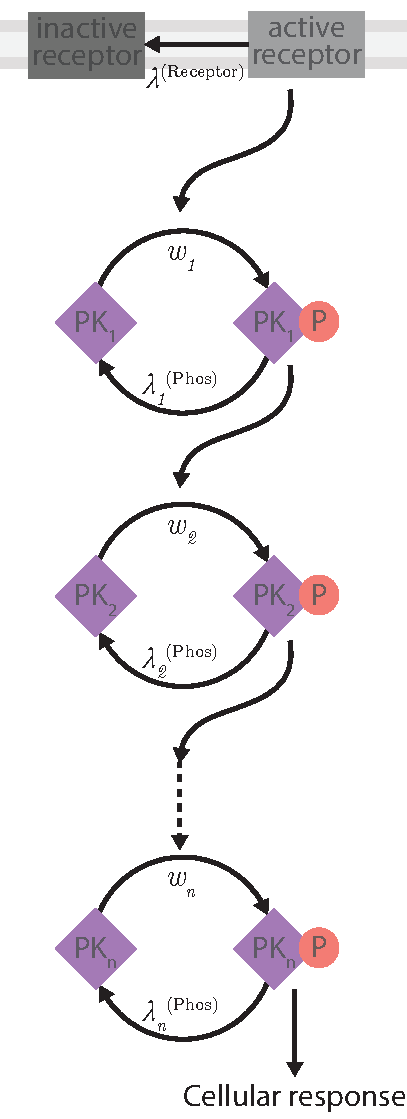
\includegraphics[width=\textwidth]{theory/fig/kinase_cascade.pdf}
\end{minipage}
\end{figure}
\end{column}
\end{columns}
\end{frame}
